\section{Profil}
\label{profile}

\begin{figure}[H]
    \begin{center}
      \frame{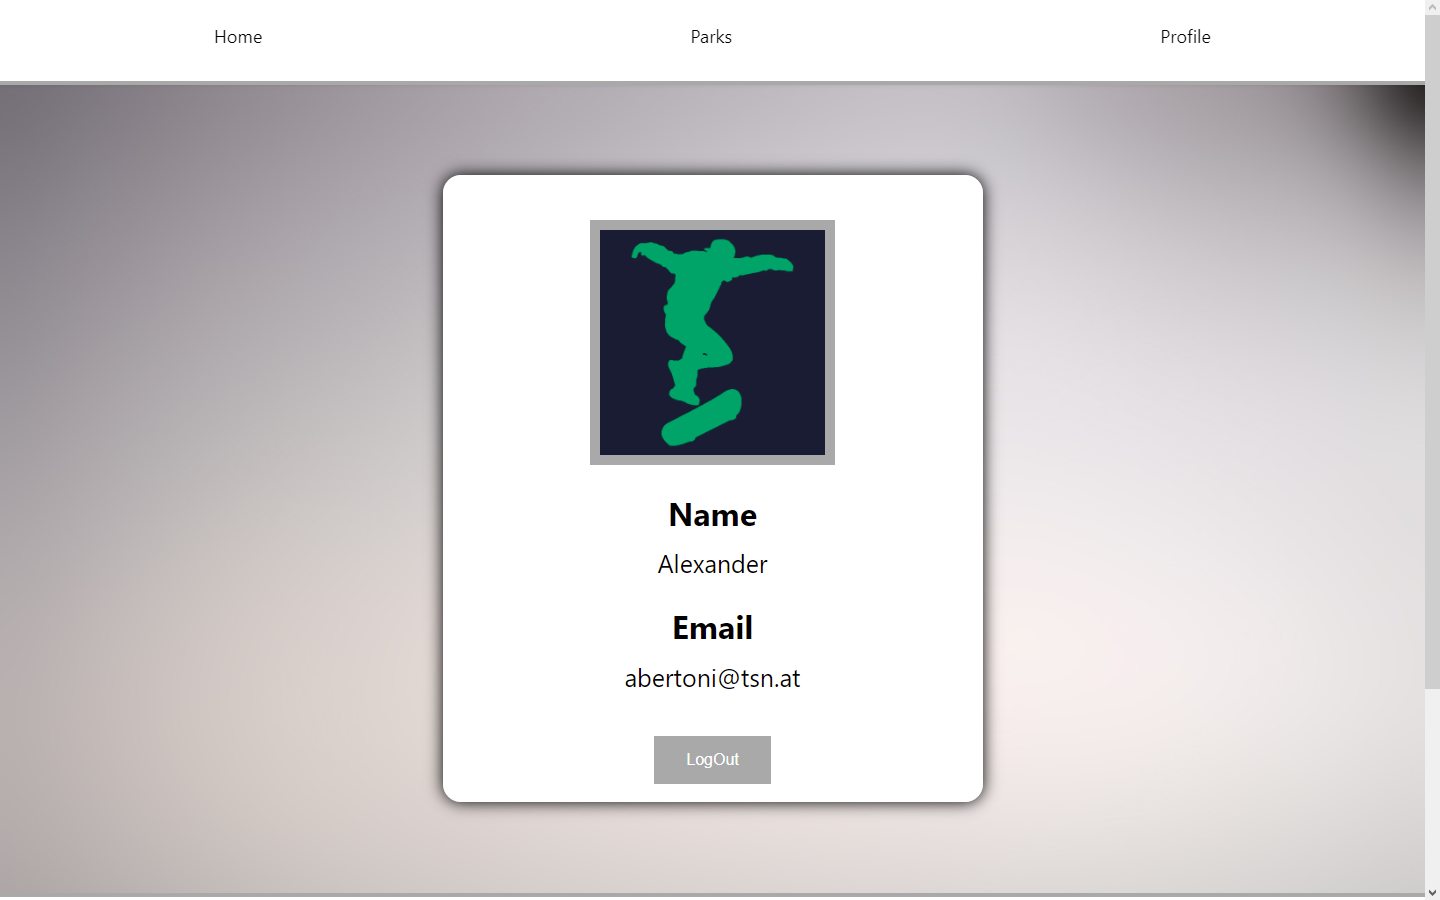
\includegraphics[width=1\textwidth]{Website/Profile.png}}
      \caption{Profil}
    \end{center}
\end{figure}

Auf der Profilseite ist es möglich seinen Benutzernamen und seine Email einzusehen. Außerdem loggt 
man sich hier von der Seite wieder aus. Die Informationen über den Benutzer werden ganz einfach über 
seinen token ausgelesen. Ist man auf der Seite nicht eingeloggt und man versucht auf die Profilseite
zu kommen indem man die URL dieser Seite eingibt, leitet diese auf die Login-view weiter. Die
Überleitung auf die Login view erfolgt wie folgt:

\begin{lstlisting}
    useEffect(() => {
        if(!sessionStorage.getItem("data")){
            navigate("/LogIn");
        }
      });
\end{lstlisting}

UseEffect ist ein React Hook welcher ausgeführt wird, wenn die Seite einmal geladen wurde. Diese 
Überprüfung wird auch in der Admin-View der Seite verwendet. 